%% -*- mode: latex; mode: reftex; tex-main-file: "slides.tex"; reftex-default-bibliography: ("../thesis") -*-

\documentclass[total,pdf,mulab,nocolorBG]{prosper}
%\documentclass[final,total,pdf,slideColor,mulab,colorBG]{prosper}
%\usepackage[mulab,highlight,toc,notes]{HA-prosper}

\RequirePackage[italian]{babel}
\usepackage[latin1]{inputenc}
\usepackage{amsmath}
\usepackage{rotating}
\usepackage{natbib}
\usepackage{xspace}
\usepackage{verbatim}
\usepackage{pstricks,pst-node,pst-text,pst-3d}
\usepackage{graphicx}
\usepackage{subfigure}



\bibpunct[, ]{[}{]}{,}{n}{,}{,}
\bibliographystyle{plainnat}

\newrgbcolor{mulablight}{0.29 0.53 0.85}
\renewcommand{\sbodycolor}{\black}
\renewcommand{\stitlecolor}{\black}
\renewcommand{\sfootcolor}{\black}
\renewcommand{\firstslidebodycolor}{\black}
\renewcommand{\firstslidetitlecolor}{\black}
\renewcommand{\firstslidesubtitlecolor}{\black}


\newcommand{\newtextcommand}[2]{\newcommand{#1}{\begingroup#2\endgroup\xspace}}
\newcommand{\renewtextcommand}[2]{\renewcommand{#1}{\begingroup#2\endgroup\xspace}}
\newcommand{\providetextcommand}[2]{\providecommand{#1}{\begingroup#2\endgroup\xspace}}

\renewcommand{\emph}[1]{\bgroup\itshape#1\egroup}

\graphicspath{
  {figures/}
}

\title{La Sintesi ad Alto Livello: \\ Estensioni al Force Directed Scheduling}
\subtitle{}
\author{Marco Lattuada}
\theday{26}{07}{2006}
\email{}
\advisor{Prof. Fabrizio Ferrandi}
\coadvisor{}


\DefaultTransition{Replace}


\begin{document}

\maketitlemulab

\begin{slide}{Obiettivo}


Modificare il Force Directed Scheduling proposto da Paulin e Knight:
\begin{itemize}
\item 
migliorando la qualit� dei risultati;
\item
diminuendo la complessit� temporale dell'algoritmo;
\item
estendendo il campo di applicabilit� dell'algoritmo aggiungendo la possibilit� di:
\begin{itemize}
\item introdurre vincoli sul numero di unit� funzionali;
\item eseguire il binding sul tipo di risorsa.
\end{itemize}
\end{itemize}

\end{slide}

\begin{slide}{La Sintesi ad Alto Livello}
\begin{itemize}
\item Sintesi ad Alto Livello: trasformazione di una descrizione comportamentale del sistema in una descrizione a livello RT;
\item Allocazione, Scheduling e Binding sono alcune delle sue fasi;
\item queste tre fasi possono essere contemporanee o successive;
\item Force Directed Originale: Allocazione + Scheduling
\item Force Directed Proposto: Allocazione + Scheduling + Binding (parziale)
\end{itemize}
\end{slide}

\include{scheduling2}
\begin{slide}{Il Force Directed Scheduling originale}
\begin{itemize}
\item Algoritmo proposto da P. G. Paulin e J. P. Knight nel 1987;
\item fissato il tempo di esecuzione minimizza il numero di risorse;
\item cerca di distribuire uniformemente le operazioni:
\begin{itemize}
\item associa ad ogni coppia <operazione-passo di controllo> una forza;
\item la forza � un numero razionale indice degli effetti dell'assegnamento;
\item ad ogni iterazione esegue l'assegnamento con forza minore (cio� migliore).
\end{itemize}
\end{itemize}
\end{slide}

\begin{slide}{Dati del Problema}
\begin{itemize}
\item SDG (\emph{System Dependence Graph}) : grafo con sia dipendenze-dato sia dipendenze di controllo;
\item Scheduling prodotto da ASAP e ALAP, finestra temporale e mobilit� di ogni operazione;
\item caratteristiche delle unit� funzionali: 
\begin{itemize}
\item tipo di operazioni eseguibili;
\item tempo di esecuzione;
\item presenza di pipeline;
\item numero di unit� (in caso di presenza di vincoli).
\end{itemize}
\end{itemize}
\end{slide}

\include{forza}
\begin{slide}{Estensioni alla versione base}
Paulin e Knight hanno proposto delle estensioni che permettono di considerare:
\begin{itemize}
\item costrutti ciclici e costrutti condizionali;
\item minimizzazione di bus e registri;
\item costo delle diverse unit� funzionali;
\item scheduling con chaining, con operazioni multiciclo, con unit� funzionali dotate di pipeline;
\item presenza di vincoli sul numero di risorse (escludendo vincoli temporali);
\item presenza di vincoli temporali locali.
\end{itemize}
\end{slide}

\begin{slide}{Limiti insiti nel Force Directed}
\begin{itemize}
\item Presenza di pi� predecessori/successori dello stesso tipo
\begin{center}
\fbox{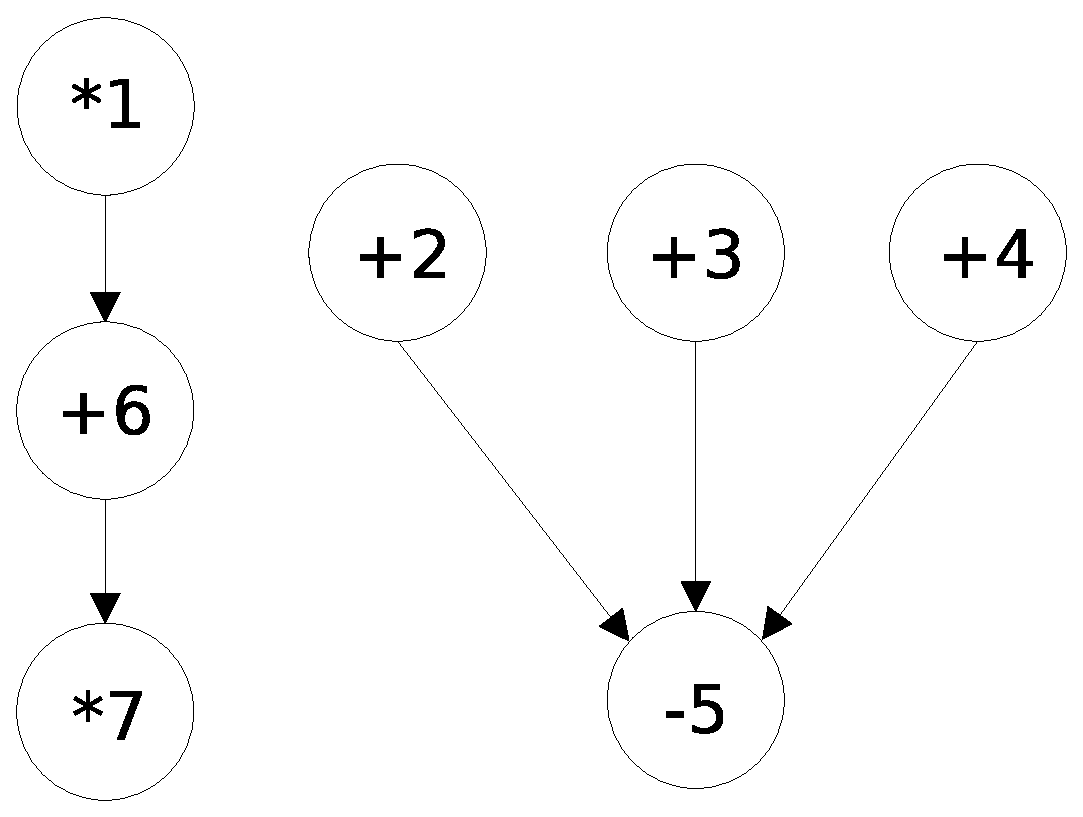
\includegraphics[scale = 0.20]{Diagram1.eps}}
\fbox{\includegraphics[scale = 0.20]{Diagram3.eps}}
\end{center}
\item Presenza di costrutti condizionali
\begin{center}
\fbox{\includegraphics[scale = 0.20]{Diagram5.eps}}
\fbox{\includegraphics[scale = 0.20]{Diagram7.eps}}
\end{center}
\end{itemize}

\end{slide}

\begin{slide}{Modifiche applicate:}
\begin{itemize}
\item formula per il calcolo della forza;
\item riduzione del peso relativo alle forze negative di predecessori e successori;
\item criterio di scelta del prossimo assegnamento da effettuare;
\item riduzione della complessit� temporale dell'algoritmo tramite scheduling a blocchi;
\item utilizzo contemporaneo di vincoli sul numero di risorse e vincoli temporali;
\item binding sul tipo di unit� funzionale.
\end{itemize}

\end{slide}

\include{modForza}
\include{modForza2}
\include{nextassign}
\include{complessita}
\begin{slide}{Utilizzo contemporaneo di due tipi di vincoli}
\begin{itemize}
\item Gli algoritmi di scheduling a tempo di esecuzione vincolato solitamente non consentono di vincolare il numero delle risorse;
\item il numero delle risorse � la funzione obiettivo da minimizzare;
\item nell'algoritmo proposto � possibile utilizzare entrambi i tipi di vincoli;
\item le motivazioni sono
\begin{itemize}
\item individuare unit� non utilizzate;
\item minimizzare il numero di risorse non vincolate;
\item minimizzare il numero di interconnessioni o di registri;
\item uniformare l'utilizzo delle risorse nei diversi passi di controllo.
\end{itemize}
\end{itemize}


\end{slide}

\include{modVincoli}
\begin{slide}{Albero di ricerca e tagli}
\begin{itemize}
\item lo scheduling con vincoli pu� essere modellizzato come esplorazione di un albero di ricerca:
\begin{itemize}
\item ogni nodo corrisponde ad una soluzione parziale;
\item ogni arco corrisponde ad un assegnamento;
\end{itemize}
\item � possibile ridurre il tempo di ricerca di una soluzione accettabile tramite:
\begin{itemize}
\item il taglio di sottoalberi il cui nodo radice corrisponda ad una soluzione esplicitamente o implicitamente non accettabile;
\item l'anticipazione di assegnamenti obbligatori;
\item backtracking anticipato;
\item riduzione del grado dell'albero di ricerca.
\end{itemize}
\end{itemize}
\end{slide}

\begin{slide}{Binding sul tipo di unita' funzionale}
\begin{itemize}
\item E' stata aggiunta la funzione di binding di un'operazione su un tipo di unit� funzionale;
\item si associa una forza ad \red ogni terna <operazione-passo di controllo-tipo di unit� funzionale> \black;
\item $FORCE(o,s,t) = self\_force(o,s,t) + pred\&succ\_force(o,s,t) + \red assign\_force(o,s,t) \black$
\item al concetto di probabilit� di un'operazione di essere schedulata in un passo di controllo si sostituisce quello di \red percentuale di occupazione di un tipo di unit� funzionale in un passo di controllo da parte di un'operazione \black;
\item in caso di mancanza di binding la nuova formulazione coincide con quella originale; 
\item � possibile utilizzare questa formulazione per tutte le casistiche del problema di scheduling.
\end{itemize}
\end{slide}

\begin{slide}{Dimensioni dei benchmark}
\begin{center}
\begin{tabular}{|l|c|c|}
\hline
Benchmark & nOp & n� salti\\
\hline
Adpcm\_decode & 68 & 11 \\
Adpcm\_encode & 83 & 14 \\
Arf & 34 & 0 \\
Bandpass & 52 & 0 \\
Chemical & 38 & 0 \\
Dct & 58 & 0 \\
Dct\_wang & 57 & 0 \\
Diffeq & 27 & 1 \\
Kim & 34 & 2 \\
Maha & 30 & 5 \\
\hline
\end{tabular}
\end{center}
\end{slide}

\begin{slide}{Risultati Sperimentali vs FD Originale}
\begin{center}
nFu indica il numero complessivo di risorse allocate: l'algoritmo non discrimina fra i diversi tipi di unit� non avendo informazioni relative ai costi\\
\begin{tabular}{|l|c c|c c|}
\hline
Benchmark & \multicolumn{2}{c|}{FD Orig.} & \multicolumn{2}{c|}{FD Modif1.} \\
& nFU & tempo & nFU & tempo \\
\hline
Adpcm\_decode & 27 & 2.89 & 18 & 10.69 \\
Adpcm\_encode & 27 & 5.84 & 19 & 43.68 \\
Arf & 14 & 0.23 & 8 & 0.25 \\
Bandpass & 20 & 0.55 & 11 & 0.57 \\
Chemical & 25 & 0.45 & 15 & 0.69 \\
Dct & 35 & 0.80 & 20 & 1.03 \\
Dct\_wang & 29 & 0.65 & 20 & 0.85 \\
Diffeq & 14 & 0.09 & 8 & 0.29 \\
\hline
\end{tabular}
\end{center}

\end{slide}

\begin{slide}{Risultati Sperimentali: Complessita'}
\begin{center}
Riduzione del tempo di computazione a seguito della riduzione di complessit�\\
\begin{tabular}{|l|c c|c c|}
\hline
Benchmark & \multicolumn{2}{c|}{FD Modif1.} & \multicolumn{2}{c|}{FD Modif2.} \\
& nFU & tempo & nFU & tempo \\
\hline
Adpcm\_decode & 18 & 11.77 & 18 & 3.54 \\
Adpcm\_encode & 19 & 43.30 & 19 & 7.92 \\
Diffeq & 8 & 0.28 & 8 & 0.25 \\
Kim & 6 & 0.68 & 6 & 0.58 \\
Maha & 5 & 0.41 & 5 & 0.25 \\
\hline
\end{tabular}
\end{center}
\end{slide}

\begin{slide}{Risultati Sperimentali vs List-Based}
\begin{center}
Guadagno in termini di unit� funzionali allocate vincolate
\begin{tabular}{|l|c||c|c||c|c|}
\hline
\multicolumn{2}{|c||}{} & \multicolumn{2}{|c||}{Kim}&  \multicolumn{2}{|c|}{Maha} \\
\hline
Unit� Funzionale & Vincolo & LB & FD & LB & FD \\
\hline
CMP &2 & & & 2 & 1 \\
indirect\_ref & inf & 1 & 2 & 1 & 1 \\
MINUS & 2 & 2 & 1 & 2 & 1 \\
PLUS & 2 & 2 & 2 & 1 & 1 \\
READ\_COND & inf & 1 & 1 & 2 & 1 \\
\hline
\multicolumn{2}{|l||}{Tempo computazione} & 0.11 & 0.18 & 0.14 & 0.12 \\
\hline
\end{tabular}
\end{center}
\end{slide}
\include{bench3}
\begin{slide}{Conclusioni e Futuri Sviluppi}
\textbf{\underline{Conclusioni} }\\
La versione proposta dell'algoritmo:
\begin{itemize}
\item ha complessit� inferiore a quella originale;
\item fornisce risultati qualitativamente migliori di quella originale;
\item permette l'introduzione di vincoli sul numero delle risorse;
\item svolge anche il binding delle operazioni sui tipi di unit� funzionali.
\end{itemize}
\textbf{\underline{Futuri Sviluppi:} }\\
\begin{itemize}
\item ridurre la complessit� in caso di assenza di costrutti di controllo;
\item minimizzazione del costo di registri e interconnessioni;
\item inserire informazioni relative al costo delle unit� funzionali;
\item valutare il guadagno dovuto ad un calcolo pi� preciso delle forze;
\item ridurre il tempo di computazione a scapito della memoria utilizzata.
\end{itemize}


\end{slide}


\end{document}
